% Options for packages loaded elsewhere
\PassOptionsToPackage{unicode}{hyperref}
\PassOptionsToPackage{hyphens}{url}
\documentclass[
]{article}
\usepackage{xcolor}
\usepackage[margin=1in]{geometry}
\usepackage{amsmath,amssymb}
\setcounter{secnumdepth}{-\maxdimen} % remove section numbering
\usepackage{iftex}
\ifPDFTeX
  \usepackage[T1]{fontenc}
  \usepackage[utf8]{inputenc}
  \usepackage{textcomp} % provide euro and other symbols
\else % if luatex or xetex
  \usepackage{unicode-math} % this also loads fontspec
  \defaultfontfeatures{Scale=MatchLowercase}
  \defaultfontfeatures[\rmfamily]{Ligatures=TeX,Scale=1}
\fi
\usepackage{lmodern}
\ifPDFTeX\else
  % xetex/luatex font selection
\fi
% Use upquote if available, for straight quotes in verbatim environments
\IfFileExists{upquote.sty}{\usepackage{upquote}}{}
\IfFileExists{microtype.sty}{% use microtype if available
  \usepackage[]{microtype}
  \UseMicrotypeSet[protrusion]{basicmath} % disable protrusion for tt fonts
}{}
\makeatletter
\@ifundefined{KOMAClassName}{% if non-KOMA class
  \IfFileExists{parskip.sty}{%
    \usepackage{parskip}
  }{% else
    \setlength{\parindent}{0pt}
    \setlength{\parskip}{6pt plus 2pt minus 1pt}}
}{% if KOMA class
  \KOMAoptions{parskip=half}}
\makeatother
\usepackage{color}
\usepackage{fancyvrb}
\newcommand{\VerbBar}{|}
\newcommand{\VERB}{\Verb[commandchars=\\\{\}]}
\DefineVerbatimEnvironment{Highlighting}{Verbatim}{commandchars=\\\{\}}
% Add ',fontsize=\small' for more characters per line
\usepackage{framed}
\definecolor{shadecolor}{RGB}{248,248,248}
\newenvironment{Shaded}{\begin{snugshade}}{\end{snugshade}}
\newcommand{\AlertTok}[1]{\textcolor[rgb]{0.94,0.16,0.16}{#1}}
\newcommand{\AnnotationTok}[1]{\textcolor[rgb]{0.56,0.35,0.01}{\textbf{\textit{#1}}}}
\newcommand{\AttributeTok}[1]{\textcolor[rgb]{0.13,0.29,0.53}{#1}}
\newcommand{\BaseNTok}[1]{\textcolor[rgb]{0.00,0.00,0.81}{#1}}
\newcommand{\BuiltInTok}[1]{#1}
\newcommand{\CharTok}[1]{\textcolor[rgb]{0.31,0.60,0.02}{#1}}
\newcommand{\CommentTok}[1]{\textcolor[rgb]{0.56,0.35,0.01}{\textit{#1}}}
\newcommand{\CommentVarTok}[1]{\textcolor[rgb]{0.56,0.35,0.01}{\textbf{\textit{#1}}}}
\newcommand{\ConstantTok}[1]{\textcolor[rgb]{0.56,0.35,0.01}{#1}}
\newcommand{\ControlFlowTok}[1]{\textcolor[rgb]{0.13,0.29,0.53}{\textbf{#1}}}
\newcommand{\DataTypeTok}[1]{\textcolor[rgb]{0.13,0.29,0.53}{#1}}
\newcommand{\DecValTok}[1]{\textcolor[rgb]{0.00,0.00,0.81}{#1}}
\newcommand{\DocumentationTok}[1]{\textcolor[rgb]{0.56,0.35,0.01}{\textbf{\textit{#1}}}}
\newcommand{\ErrorTok}[1]{\textcolor[rgb]{0.64,0.00,0.00}{\textbf{#1}}}
\newcommand{\ExtensionTok}[1]{#1}
\newcommand{\FloatTok}[1]{\textcolor[rgb]{0.00,0.00,0.81}{#1}}
\newcommand{\FunctionTok}[1]{\textcolor[rgb]{0.13,0.29,0.53}{\textbf{#1}}}
\newcommand{\ImportTok}[1]{#1}
\newcommand{\InformationTok}[1]{\textcolor[rgb]{0.56,0.35,0.01}{\textbf{\textit{#1}}}}
\newcommand{\KeywordTok}[1]{\textcolor[rgb]{0.13,0.29,0.53}{\textbf{#1}}}
\newcommand{\NormalTok}[1]{#1}
\newcommand{\OperatorTok}[1]{\textcolor[rgb]{0.81,0.36,0.00}{\textbf{#1}}}
\newcommand{\OtherTok}[1]{\textcolor[rgb]{0.56,0.35,0.01}{#1}}
\newcommand{\PreprocessorTok}[1]{\textcolor[rgb]{0.56,0.35,0.01}{\textit{#1}}}
\newcommand{\RegionMarkerTok}[1]{#1}
\newcommand{\SpecialCharTok}[1]{\textcolor[rgb]{0.81,0.36,0.00}{\textbf{#1}}}
\newcommand{\SpecialStringTok}[1]{\textcolor[rgb]{0.31,0.60,0.02}{#1}}
\newcommand{\StringTok}[1]{\textcolor[rgb]{0.31,0.60,0.02}{#1}}
\newcommand{\VariableTok}[1]{\textcolor[rgb]{0.00,0.00,0.00}{#1}}
\newcommand{\VerbatimStringTok}[1]{\textcolor[rgb]{0.31,0.60,0.02}{#1}}
\newcommand{\WarningTok}[1]{\textcolor[rgb]{0.56,0.35,0.01}{\textbf{\textit{#1}}}}
\usepackage{graphicx}
\makeatletter
\newsavebox\pandoc@box
\newcommand*\pandocbounded[1]{% scales image to fit in text height/width
  \sbox\pandoc@box{#1}%
  \Gscale@div\@tempa{\textheight}{\dimexpr\ht\pandoc@box+\dp\pandoc@box\relax}%
  \Gscale@div\@tempb{\linewidth}{\wd\pandoc@box}%
  \ifdim\@tempb\p@<\@tempa\p@\let\@tempa\@tempb\fi% select the smaller of both
  \ifdim\@tempa\p@<\p@\scalebox{\@tempa}{\usebox\pandoc@box}%
  \else\usebox{\pandoc@box}%
  \fi%
}
% Set default figure placement to htbp
\def\fps@figure{htbp}
\makeatother
\setlength{\emergencystretch}{3em} % prevent overfull lines
\providecommand{\tightlist}{%
  \setlength{\itemsep}{0pt}\setlength{\parskip}{0pt}}
\usepackage{bookmark}
\IfFileExists{xurl.sty}{\usepackage{xurl}}{} % add URL line breaks if available
\urlstyle{same}
\hypersetup{
  pdftitle={MA213 Basic Statistics and Probability - Lab1 Guide},
  hidelinks,
  pdfcreator={LaTeX via pandoc}}

\title{MA213 Basic Statistics and Probability - Lab1 Guide}
\author{}
\date{\vspace{-2.5em}}

\begin{document}
\maketitle

\subsection{\texorpdfstring{\textbf{Lab 1: Introduction to
R}}{Lab 1: Introduction to R}}\label{lab-1-introduction-to-r}

In this lab session, we will learn basic syntax of R.

\subsection{Learning Objectives}\label{learning-objectives}

\begin{itemize}
\tightlist
\item
  Use R for Data Management and Exploration: Utilize R to load,
  pre-process, and explore data through visualization and summarization
  techniques.
\end{itemize}

\paragraph{Install R and RStudio.}\label{install-r-and-rstudio.}

You can download and install R from

\url{https://www.r-project.org/}

And you can download and install RStudio from

\url{https://posit.co/download/rstudio-desktop/}

We assume that you have already installed R and Rstudio (You need to
install first R and then install Rstudio because Rstudio is an IDE for
R).

\subsection{Introduction of R}\label{introduction-of-r}

\begin{itemize}
\item
  R is Programming language and environment statistical computing, data
  manipulation and graphical display.
\item
  R is free and open source.
\item
  Rstudio is also free and open source IDE (Integrated Development
  Environment) for R.
\end{itemize}

\subsection{Brief walk through about RStudio
interface}\label{brief-walk-through-about-rstudio-interface}

\begin{figure}
\centering
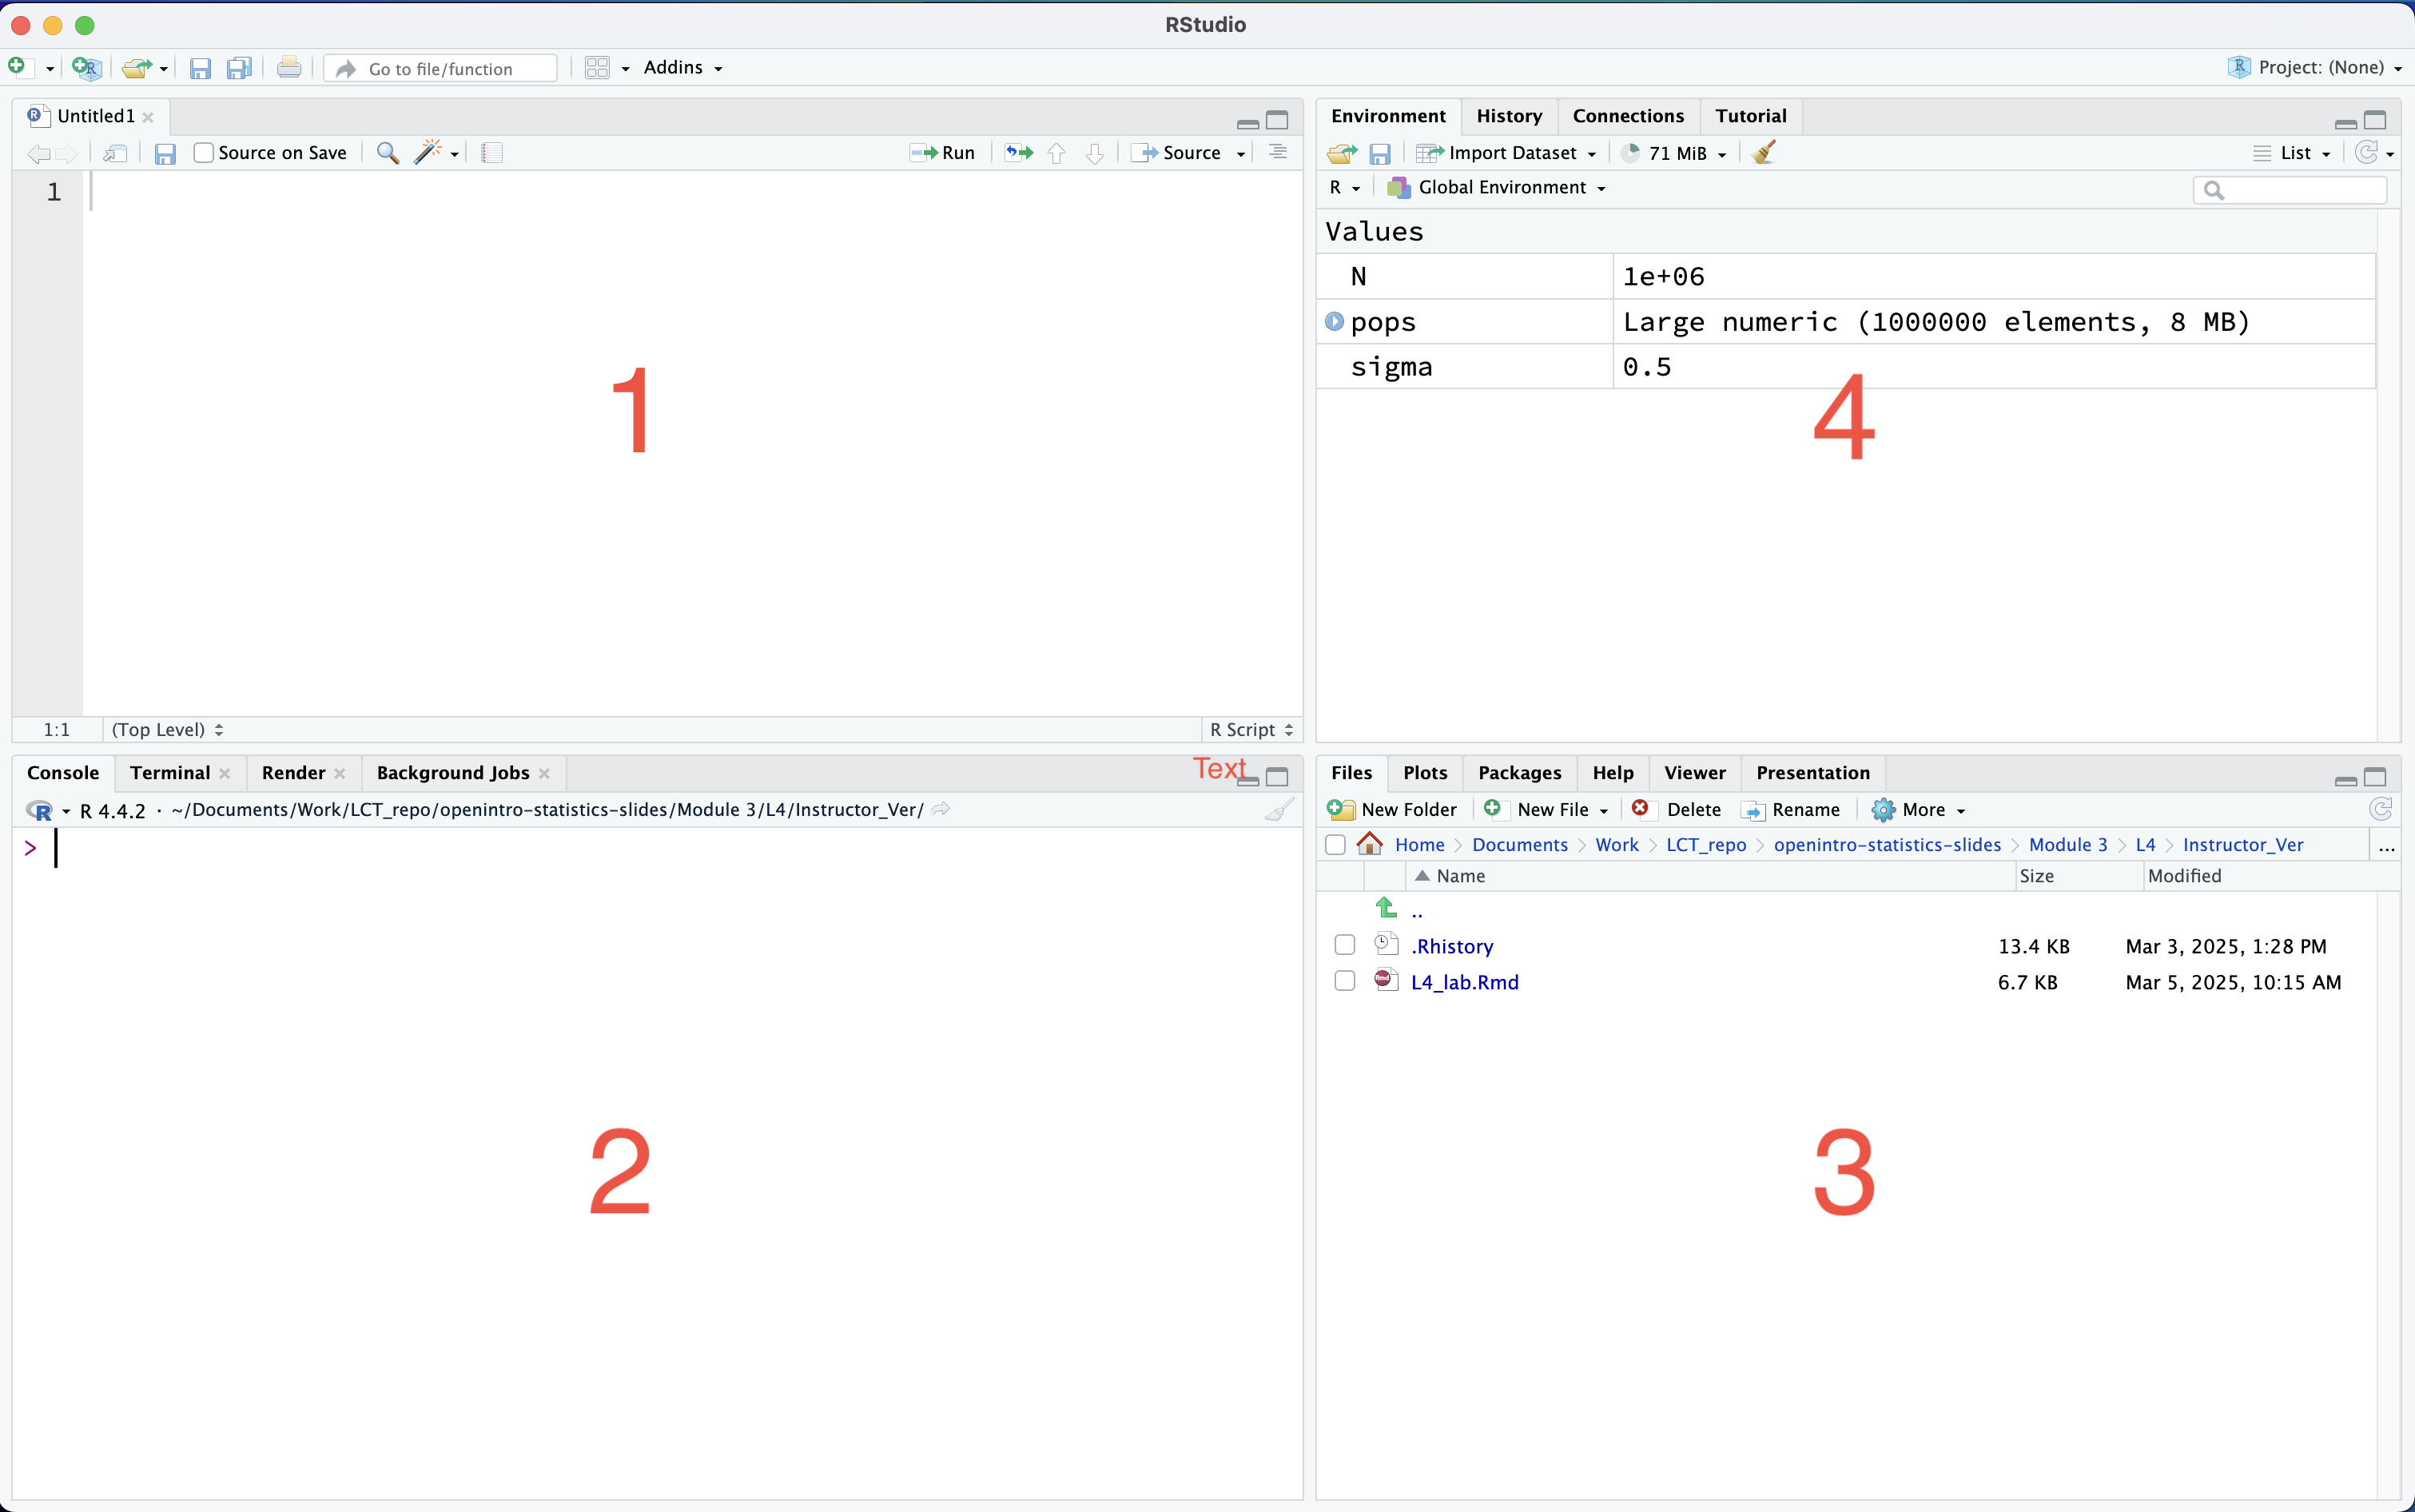
\includegraphics[width=7.98958in,height=\textheight,keepaspectratio]{lab1/images/Screen_Shot_Rstudio.png}
\caption{RStudio overview}
\end{figure}

window \texttt{1} : script window (text editor)

window \texttt{2} : console window (this is where you type your R code
and run)

window \texttt{3} : plots, files, packages, help\ldots{} window

window \texttt{4} : environment window

\subsection{\texorpdfstring{Set up
\texttt{working\ directory}}{Set up working directory}}\label{set-up-working-directory}

\begin{itemize}
\item
  You can go to \texttt{Session} → \texttt{set\ working\ directory} →
  \texttt{choose\ directory} and then choose your working directory.

  or
\item
  You can go to \texttt{Files} tap → ☸︎ →`copy folder path to Clipboard'

  then paste into \texttt{setwd()} function
\end{itemize}

or

\begin{itemize}
\tightlist
\item
  You can go to \texttt{Files} tap → ☸︎ →`Set As Working Directory'
\end{itemize}

\subsection{How to run code?}\label{how-to-run-code}

\begin{enumerate}
\def\labelenumi{\arabic{enumi}.}
\item
  Directly type your command in the console window.
\item
  You can run your R chunk by pressing run button \texttt{▶} in the R
  chunk in your R markdown file.
\item
  You can write your commands on your R script file and highlight the
  commands and press \texttt{run}
\end{enumerate}

\begin{verbatim}
Run shortcut : `ctrl` + `enter` (windows) or `cmd` + `enter` (mac).
\end{verbatim}

\subsection{R is basically a big calculator (some mathematics) : basic
math operations to matrix
operations}\label{r-is-basically-a-big-calculator-some-mathematics-basic-math-operations-to-matrix-operations}

\begin{quote}
\begin{itemize}
\tightlist
\item
  Basic math operations
\end{itemize}

\texttt{+}: add

\texttt{-} : substract

\texttt{*} : multiply

\texttt{/} : divide

\texttt{\^{}} or \texttt{**}: exponent
\end{quote}

\subsection{For example}\label{for-example}

\((\frac{12}{24})^2\)

\begin{Shaded}
\begin{Highlighting}[]
\NormalTok{(}\DecValTok{12}\SpecialCharTok{/}\DecValTok{24}\NormalTok{)}\SpecialCharTok{\^{}}\NormalTok{(}\DecValTok{2}\NormalTok{)}
\end{Highlighting}
\end{Shaded}

\begin{verbatim}
## [1] 0.25
\end{verbatim}

\begin{Shaded}
\begin{Highlighting}[]
\CommentTok{\#or}
\NormalTok{(}\DecValTok{12}\SpecialCharTok{/}\DecValTok{24}\NormalTok{)}\SpecialCharTok{**}\NormalTok{(}\DecValTok{2}\NormalTok{)}
\end{Highlighting}
\end{Shaded}

\begin{verbatim}
## [1] 0.25
\end{verbatim}

\subsection{Assign values to a
variable}\label{assign-values-to-a-variable}

Let's say if you want to save 10 to variable \texttt{A}. You can do the
following command.

\begin{Shaded}
\begin{Highlighting}[]
\NormalTok{A }\OtherTok{\textless{}{-}} \DecValTok{10}
\NormalTok{A }\OtherTok{\textless{}\textless{}{-}} \DecValTok{10}
\DecValTok{10} \OtherTok{{-}\textgreater{}}\NormalTok{ A}
\DecValTok{10} \OtherTok{{-}\textgreater{}\textgreater{}}\NormalTok{ A}
\NormalTok{A }\OtherTok{=} \DecValTok{10}

\CommentTok{\# A \textless{}{-} 10}
\CommentTok{\# A = 10 }
\CommentTok{\# commonly used ones }
\end{Highlighting}
\end{Shaded}

\subsection{\texorpdfstring{And you can check what value the variable
\texttt{A} has by calling it or using \texttt{print()}
function}{And you can check what value the variable A has by calling it or using print() function}}\label{and-you-can-check-what-value-the-variable-a-has-by-calling-it-or-using-print-function}

\begin{Shaded}
\begin{Highlighting}[]
\NormalTok{A}
\end{Highlighting}
\end{Shaded}

\begin{verbatim}
## [1] 10
\end{verbatim}

\begin{Shaded}
\begin{Highlighting}[]
\FunctionTok{print}\NormalTok{(A)}
\end{Highlighting}
\end{Shaded}

\begin{verbatim}
## [1] 10
\end{verbatim}

Assigning character type information to a variable

\begin{Shaded}
\begin{Highlighting}[]
\NormalTok{SchoolName }\OtherTok{\textless{}{-}} \StringTok{"Boston University"}
\NormalTok{SchoolName}
\end{Highlighting}
\end{Shaded}

\begin{verbatim}
## [1] "Boston University"
\end{verbatim}

\subsection{Assign values to a vector}\label{assign-values-to-a-vector}

You can assign multiple values to a vector.

\begin{Shaded}
\begin{Highlighting}[]
\NormalTok{GPA }\OtherTok{\textless{}{-}} \FunctionTok{c}\NormalTok{(}\FloatTok{3.2}\NormalTok{, }\FloatTok{3.7}\NormalTok{, }\FloatTok{3.9}\NormalTok{, }\FloatTok{2.3}\NormalTok{, }\FloatTok{2.7}\NormalTok{)}
\NormalTok{FirstName }\OtherTok{\textless{}{-}} \FunctionTok{c}\NormalTok{(}\StringTok{"Tom"}\NormalTok{, }\StringTok{"Sarah"}\NormalTok{, }\StringTok{"Nick"}\NormalTok{, }\StringTok{"Amy"}\NormalTok{, }\StringTok{"John"}\NormalTok{)}
\NormalTok{GPA}
\end{Highlighting}
\end{Shaded}

\begin{verbatim}
## [1] 3.2 3.7 3.9 2.3 2.7
\end{verbatim}

\begin{Shaded}
\begin{Highlighting}[]
\NormalTok{FirstName}
\end{Highlighting}
\end{Shaded}

\begin{verbatim}
## [1] "Tom"   "Sarah" "Nick"  "Amy"   "John"
\end{verbatim}

There are some useful functions for a vector

\begin{itemize}
\item
  \texttt{seq(from=a,\ to=b,\ by=c)} : this generates a sequence vector
  from value a to b by c increment.
\item
  \texttt{rep(x,\ times\ =\ n)} : this replicate element \texttt{x} for
  n times.
\item
  \texttt{length(x)} : this will give you the length of vector
  \texttt{x}
\end{itemize}

\subsection{Examples}\label{examples}

\begin{Shaded}
\begin{Highlighting}[]
\NormalTok{my\_vector }\OtherTok{=} \FunctionTok{seq}\NormalTok{(}\DecValTok{1}\NormalTok{, }\DecValTok{10}\NormalTok{, }\DecValTok{2}\NormalTok{)}
\NormalTok{my\_vector}
\end{Highlighting}
\end{Shaded}

\begin{verbatim}
## [1] 1 3 5 7 9
\end{verbatim}

\begin{Shaded}
\begin{Highlighting}[]
\NormalTok{another\_vector }\OtherTok{=} \DecValTok{1}\SpecialCharTok{:}\DecValTok{10}
\NormalTok{another\_vector}
\end{Highlighting}
\end{Shaded}

\begin{verbatim}
##  [1]  1  2  3  4  5  6  7  8  9 10
\end{verbatim}

\begin{Shaded}
\begin{Highlighting}[]
\NormalTok{vector3 }\OtherTok{=} \FunctionTok{rep}\NormalTok{(}\StringTok{"BU"}\NormalTok{, }\DecValTok{25}\NormalTok{)}
\NormalTok{vector3}
\end{Highlighting}
\end{Shaded}

\begin{verbatim}
##  [1] "BU" "BU" "BU" "BU" "BU" "BU" "BU" "BU" "BU" "BU" "BU" "BU" "BU" "BU" "BU"
## [16] "BU" "BU" "BU" "BU" "BU" "BU" "BU" "BU" "BU" "BU"
\end{verbatim}

\subsection{Accessing vector elements}\label{accessing-vector-elements}

Each element in a vector is associated with index number. The index in R
starts from 1 as the first item.

For example,

\begin{Shaded}
\begin{Highlighting}[]
\CommentTok{\#}
\NormalTok{SomeNames }\OtherTok{\textless{}{-}} \FunctionTok{c}\NormalTok{(}\StringTok{"Alpha"}\NormalTok{, }\StringTok{"Bravo"}\NormalTok{, }\StringTok{"Charlie"}\NormalTok{)}
\end{Highlighting}
\end{Shaded}

\begin{figure}
\centering
\pandocbounded{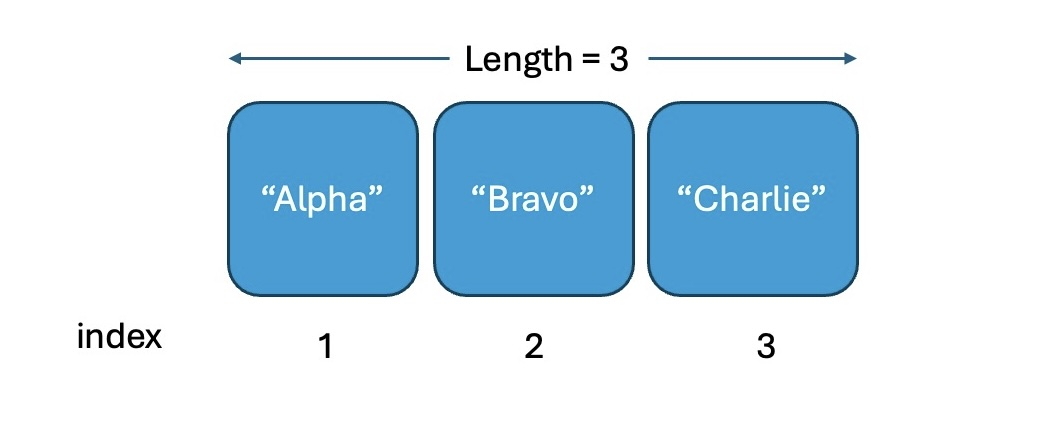
\includegraphics[keepaspectratio]{lab1/images/index.jpg}}
\caption{Index of Vector Elements}
\end{figure}

\subsection{For example}\label{for-example-1}

You can access the third element of \texttt{SomeNames} by
\texttt{SomeNames{[}3{]}} .

You can also access, for example, the second and the third elements by
\texttt{SomeNames{[}2:3{]}} .

\begin{Shaded}
\begin{Highlighting}[]
\CommentTok{\#}
\NormalTok{SomeNames[}\DecValTok{3}\NormalTok{]}
\end{Highlighting}
\end{Shaded}

\begin{verbatim}
## [1] "Charlie"
\end{verbatim}

\begin{Shaded}
\begin{Highlighting}[]
\NormalTok{SomeNames[}\DecValTok{2}\SpecialCharTok{:}\DecValTok{3}\NormalTok{]}
\end{Highlighting}
\end{Shaded}

\begin{verbatim}
## [1] "Bravo"   "Charlie"
\end{verbatim}

\subsection{Numeric vector can be subsetted using
condition}\label{numeric-vector-can-be-subsetted-using-condition}

\begin{Shaded}
\begin{Highlighting}[]
\NormalTok{                         x[condition]}
\end{Highlighting}
\end{Shaded}

the conditional statements (condition) you can use could be

\begin{Shaded}
\begin{Highlighting}[]
\NormalTok{x }\SpecialCharTok{==} \DecValTok{20}    \CommentTok{\# x equals to 20}
\NormalTok{x }\SpecialCharTok{\textless{}} \DecValTok{100}
\NormalTok{x }\SpecialCharTok{\textless{}=} \DecValTok{100}
\NormalTok{x }\SpecialCharTok{\textgreater{}} \DecValTok{100}
\NormalTok{x }\SpecialCharTok{\textgreater{}=} \DecValTok{100}
\NormalTok{x }\SpecialCharTok{!=} \DecValTok{100}   \CommentTok{\# x not equal to 100}
\end{Highlighting}
\end{Shaded}

\subsection{For example}\label{for-example-2}

\begin{Shaded}
\begin{Highlighting}[]
\NormalTok{Numbers }\OtherTok{\textless{}{-}} \FunctionTok{c}\NormalTok{(}\DecValTok{20}\NormalTok{, }\DecValTok{30}\NormalTok{, }\DecValTok{50}\NormalTok{, }\DecValTok{70}\NormalTok{, }\DecValTok{120}\NormalTok{, }\DecValTok{200}\NormalTok{)}
\NormalTok{Numbers[Numbers}\SpecialCharTok{\textless{}}\DecValTok{100}\NormalTok{]}
\end{Highlighting}
\end{Shaded}

\begin{verbatim}
## [1] 20 30 50 70
\end{verbatim}

\begin{figure}
\centering
\pandocbounded{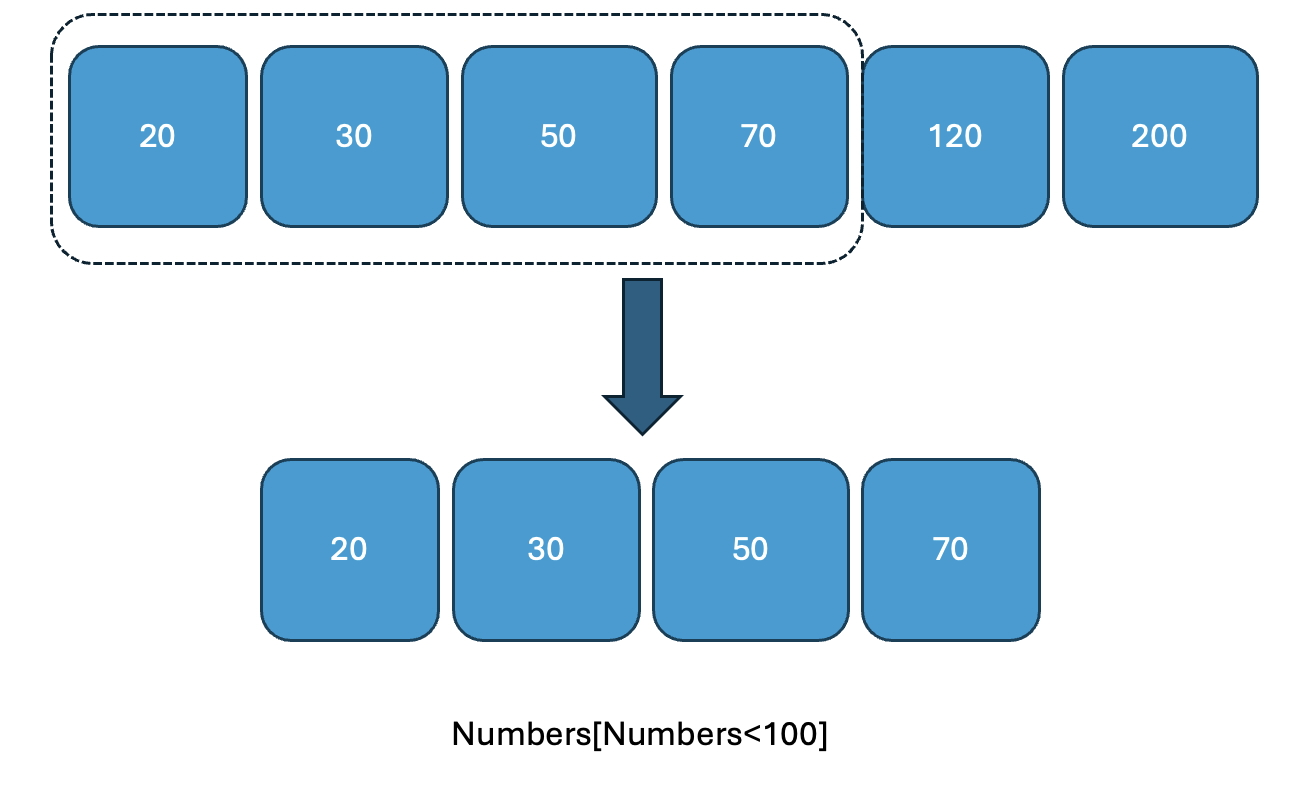
\includegraphics[keepaspectratio]{lab1/images/Slicing.jpg}}
\caption{Subsetting vector using condition}
\end{figure}

\subsection{Importing and Subsetting
Data}\label{importing-and-subsetting-data}

You can import Data by using \texttt{read.table()} function.

\begin{Shaded}
\begin{Highlighting}[]
\NormalTok{my\_data }\OtherTok{\textless{}{-}} \FunctionTok{read.csv}\NormalTok{(}\StringTok{"lab1/data/mtcars.csv"}\NormalTok{)}
\CommentTok{\# to be able to import this file, this file needs to be in your working directory}
\end{Highlighting}
\end{Shaded}

\subsection{You can access subset
data}\label{you-can-access-subset-data}

\begin{itemize}
\item
  Specific element by \texttt{my\_data{[}row,\ column{]}}

  \begin{itemize}
  \tightlist
  \item
    \textbar{} for example, the element in the third row and the fourth
    column \texttt{my\_data{[}3,4{]}}
  \end{itemize}
\item
  Specific row by \texttt{my\_data{[}row,{]}}

  \begin{itemize}
  \tightlist
  \item
    \textbar{} for example, all the element of the third row
    \texttt{my\_data{[}3,{]}}
  \end{itemize}
\end{itemize}

\subsection{Also,}\label{also}

\begin{itemize}
\item
  Specific column by \texttt{my\_data{[},column{]}}

  \begin{itemize}
  \tightlist
  \item
    \textbar{} for example, all the element of the fifth column
    \texttt{my\_data{[},5{]}}
  \end{itemize}
\item
  Access the column by using \texttt{\$} sign such as
  \texttt{my\_data\$column\_name}

  \begin{itemize}
  \tightlist
  \item
    \textbar{} for example, \texttt{hp} column from \texttt{my\_data} is
    \texttt{my\_data\$hp}
  \end{itemize}
\item
  Conditional statement works similar as vectors (row wise and column
  wise)

  \begin{itemize}
  \tightlist
  \item
    \textbar{} for example,
    \texttt{my\_data{[}my\_data\$hp\textless{}100,{]}}
  \end{itemize}
\end{itemize}

\subsection{Multiple conditions can be
combined}\label{multiple-conditions-can-be-combined}

You can combine multiple logical conditions using \& (AND), \textbar{}
(OR), and ! (NOT) operators inside the row index to filter rows. For
example

\begin{itemize}
\tightlist
\item
  Rows where \texttt{hp} is less than 100 AND \texttt{cyl} equals 4:
\end{itemize}

\begin{Shaded}
\begin{Highlighting}[]
\NormalTok{my\_data[(my\_data}\SpecialCharTok{$}\NormalTok{hp }\SpecialCharTok{\textless{}} \DecValTok{100}\NormalTok{) }\SpecialCharTok{\&}\NormalTok{ (my\_data}\SpecialCharTok{$}\NormalTok{cyl }\SpecialCharTok{==} \DecValTok{4}\NormalTok{), ]}
\end{Highlighting}
\end{Shaded}

\begin{verbatim}
##                 X  mpg cyl  disp hp drat    wt  qsec vs am gear carb
## 3      Datsun 710 22.8   4 108.0 93 3.85 2.320 18.61  1  1    4    1
## 8       Merc 240D 24.4   4 146.7 62 3.69 3.190 20.00  1  0    4    2
## 9        Merc 230 22.8   4 140.8 95 3.92 3.150 22.90  1  0    4    2
## 18       Fiat 128 32.4   4  78.7 66 4.08 2.200 19.47  1  1    4    1
## 19    Honda Civic 30.4   4  75.7 52 4.93 1.615 18.52  1  1    4    2
## 20 Toyota Corolla 33.9   4  71.1 65 4.22 1.835 19.90  1  1    4    1
## 21  Toyota Corona 21.5   4 120.1 97 3.70 2.465 20.01  1  0    3    1
## 26      Fiat X1-9 27.3   4  79.0 66 4.08 1.935 18.90  1  1    4    1
## 27  Porsche 914-2 26.0   4 120.3 91 4.43 2.140 16.70  0  1    5    2
\end{verbatim}

\begin{itemize}
\tightlist
\item
  Rows where \texttt{hp} is less than 100 OR \texttt{cyl} equals 4:
\end{itemize}

\begin{Shaded}
\begin{Highlighting}[]
\NormalTok{my\_data[my\_data}\SpecialCharTok{$}\NormalTok{hp }\SpecialCharTok{\textless{}} \DecValTok{100} \SpecialCharTok{|}\NormalTok{ my\_data}\SpecialCharTok{$}\NormalTok{cyl }\SpecialCharTok{==} \DecValTok{4}\NormalTok{, ]}
\end{Highlighting}
\end{Shaded}

\begin{verbatim}
##                 X  mpg cyl  disp  hp drat    wt  qsec vs am gear carb
## 3      Datsun 710 22.8   4 108.0  93 3.85 2.320 18.61  1  1    4    1
## 8       Merc 240D 24.4   4 146.7  62 3.69 3.190 20.00  1  0    4    2
## 9        Merc 230 22.8   4 140.8  95 3.92 3.150 22.90  1  0    4    2
## 18       Fiat 128 32.4   4  78.7  66 4.08 2.200 19.47  1  1    4    1
## 19    Honda Civic 30.4   4  75.7  52 4.93 1.615 18.52  1  1    4    2
## 20 Toyota Corolla 33.9   4  71.1  65 4.22 1.835 19.90  1  1    4    1
## 21  Toyota Corona 21.5   4 120.1  97 3.70 2.465 20.01  1  0    3    1
## 26      Fiat X1-9 27.3   4  79.0  66 4.08 1.935 18.90  1  1    4    1
## 27  Porsche 914-2 26.0   4 120.3  91 4.43 2.140 16.70  0  1    5    2
## 28   Lotus Europa 30.4   4  95.1 113 3.77 1.513 16.90  1  1    5    2
## 32     Volvo 142E 21.4   4 121.0 109 4.11 2.780 18.60  1  1    4    2
\end{verbatim}

Rows where \texttt{hp} is NOT less than 100:

\begin{Shaded}
\begin{Highlighting}[]
\NormalTok{my\_data[}\SpecialCharTok{!}\NormalTok{ (my\_data}\SpecialCharTok{$}\NormalTok{hp }\SpecialCharTok{\textless{}} \DecValTok{100}\NormalTok{), ]}
\end{Highlighting}
\end{Shaded}

\begin{verbatim}
##                      X  mpg cyl  disp  hp drat    wt  qsec vs am gear carb
## 1            Mazda RX4 21.0   6 160.0 110 3.90 2.620 16.46  0  1    4    4
## 2        Mazda RX4 Wag 21.0   6 160.0 110 3.90 2.875 17.02  0  1    4    4
## 4       Hornet 4 Drive 21.4   6 258.0 110 3.08 3.215 19.44  1  0    3    1
## 5    Hornet Sportabout 18.7   8 360.0 175 3.15 3.440 17.02  0  0    3    2
## 6              Valiant 18.1   6 225.0 105 2.76 3.460 20.22  1  0    3    1
## 7           Duster 360 14.3   8 360.0 245 3.21 3.570 15.84  0  0    3    4
## 10            Merc 280 19.2   6 167.6 123 3.92 3.440 18.30  1  0    4    4
## 11           Merc 280C 17.8   6 167.6 123 3.92 3.440 18.90  1  0    4    4
## 12          Merc 450SE 16.4   8 275.8 180 3.07 4.070 17.40  0  0    3    3
## 13          Merc 450SL 17.3   8 275.8 180 3.07 3.730 17.60  0  0    3    3
## 14         Merc 450SLC 15.2   8 275.8 180 3.07 3.780 18.00  0  0    3    3
## 15  Cadillac Fleetwood 10.4   8 472.0 205 2.93 5.250 17.98  0  0    3    4
## 16 Lincoln Continental 10.4   8 460.0 215 3.00 5.424 17.82  0  0    3    4
## 17   Chrysler Imperial 14.7   8 440.0 230 3.23 5.345 17.42  0  0    3    4
## 22    Dodge Challenger 15.5   8 318.0 150 2.76 3.520 16.87  0  0    3    2
## 23         AMC Javelin 15.2   8 304.0 150 3.15 3.435 17.30  0  0    3    2
## 24          Camaro Z28 13.3   8 350.0 245 3.73 3.840 15.41  0  0    3    4
## 25    Pontiac Firebird 19.2   8 400.0 175 3.08 3.845 17.05  0  0    3    2
## 28        Lotus Europa 30.4   4  95.1 113 3.77 1.513 16.90  1  1    5    2
## 29      Ford Pantera L 15.8   8 351.0 264 4.22 3.170 14.50  0  1    5    4
## 30        Ferrari Dino 19.7   6 145.0 175 3.62 2.770 15.50  0  1    5    6
## 31       Maserati Bora 15.0   8 301.0 335 3.54 3.570 14.60  0  1    5    8
## 32          Volvo 142E 21.4   4 121.0 109 4.11 2.780 18.60  1  1    4    2
\end{verbatim}

\subsubsection{\texorpdfstring{If an expression or condition is True or
False, programming language gives two answers \texttt{TRUE} or
\texttt{FALSE} . It is sometimes can be shown to \texttt{1} or
\texttt{0}.}{If an expression or condition is True or False, programming language gives two answers TRUE or FALSE . It is sometimes can be shown to 1 or 0.}}\label{if-an-expression-or-condition-is-true-or-false-programming-language-gives-two-answers-true-or-false-.-it-is-sometimes-can-be-shown-to-1-or-0.}

\begin{Shaded}
\begin{Highlighting}[]
\DecValTok{3}\SpecialCharTok{==}\DecValTok{3} \CommentTok{\# True}
\end{Highlighting}
\end{Shaded}

\begin{verbatim}
## [1] TRUE
\end{verbatim}

\begin{Shaded}
\begin{Highlighting}[]
\DecValTok{10} \SpecialCharTok{==} \DecValTok{3} \CommentTok{\# False}
\end{Highlighting}
\end{Shaded}

\begin{verbatim}
## [1] FALSE
\end{verbatim}

\begin{Shaded}
\begin{Highlighting}[]
\NormalTok{my\_data}\SpecialCharTok{$}\NormalTok{hp }\SpecialCharTok{\textless{}} \DecValTok{100} \CommentTok{\# if the horse power of the car is less than 100 it gives 1, 0 otherwise. }
\end{Highlighting}
\end{Shaded}

\begin{verbatim}
##  [1] FALSE FALSE  TRUE FALSE FALSE FALSE FALSE  TRUE  TRUE FALSE FALSE FALSE
## [13] FALSE FALSE FALSE FALSE FALSE  TRUE  TRUE  TRUE  TRUE FALSE FALSE FALSE
## [25] FALSE  TRUE  TRUE FALSE FALSE FALSE FALSE FALSE
\end{verbatim}

\begin{Shaded}
\begin{Highlighting}[]
\NormalTok{my\_data[my\_data}\SpecialCharTok{$}\NormalTok{hp }\SpecialCharTok{\textless{}} \DecValTok{100}\NormalTok{,] }\CommentTok{\# this is how we are only printing the cars data with horse power \textless{} 100. }
\end{Highlighting}
\end{Shaded}

\begin{verbatim}
##                 X  mpg cyl  disp hp drat    wt  qsec vs am gear carb
## 3      Datsun 710 22.8   4 108.0 93 3.85 2.320 18.61  1  1    4    1
## 8       Merc 240D 24.4   4 146.7 62 3.69 3.190 20.00  1  0    4    2
## 9        Merc 230 22.8   4 140.8 95 3.92 3.150 22.90  1  0    4    2
## 18       Fiat 128 32.4   4  78.7 66 4.08 2.200 19.47  1  1    4    1
## 19    Honda Civic 30.4   4  75.7 52 4.93 1.615 18.52  1  1    4    2
## 20 Toyota Corolla 33.9   4  71.1 65 4.22 1.835 19.90  1  1    4    1
## 21  Toyota Corona 21.5   4 120.1 97 3.70 2.465 20.01  1  0    3    1
## 26      Fiat X1-9 27.3   4  79.0 66 4.08 1.935 18.90  1  1    4    1
## 27  Porsche 914-2 26.0   4 120.3 91 4.43 2.140 16.70  0  1    5    2
\end{verbatim}

\end{document}
